\documentclass{subfiles}

\begin{document}
    \marginnote{\textit{\textbf{VL 17}}\\26.06.2023\\11:45}

    Um die Wechselwirkung des Spins mit dem Magnetfeld zu beschreiben, wechseln wir in die semiklassische Betrachtungsperspektive. Gehe hierzu über in das Bezugssystem des Elektrons. Für eine mit Strom $I$ durchflossene Kurve mit eingeschlossener Fläche $A$ ergibt sich nach Biot Savart das Magnetfeld
    \[
        B = \fdef{\frac{\mu_0}{4\pi}\cdot\frac{I}{r^3}\cdot A}{r\in\R^3} = \fdef{
            \frac{\mu_0\cdot Ze}{4\pi\cdot \dabs{r}{2}^3}\cdot(v \times r)
        }{r\in\R^3}
    \]
    mit $v\in\R^3$ als Rotationsgeschwindigkeit. Wir arbeiten jedoch hier nur ungefähr, denn die Hin- und Rücktransformation ist in relativistischer Anschauung nicht trivial. 
    \begin{Aufgabe}
        \nr{} Führe die Berechnung unter Berücksichtigung der Lorentz Transformation durch. Verifiziere den Zusammenhang der beiden Lösungen durch den Faktor $1/2$ (\href{https://en.wikipedia.org/wiki/Thomas_precession}{\emph{Thomas Faktor}}). 

        \nr{} Bestimme die Formel für das elektrische Feld: $\Delta E_{l,s}(r) \approx \frac{\mu_0\cdot Ze^2}{8\pi m_e^2\cdot \dabs{r}{2}^3}\cdot(\scpr{s}{l})$.
    \end{Aufgabe}
    Daraus ergibt sich der um den Spin erweiterten Hamiltonoperator
    \[
        H_{V,S,n}:=\fdef{\frac{P_n^2(x)}{2m} + V(Q_n)(x) + \sum_{i\in[d]}(S_i\cdot J_i)(x)}{x\in\mcH},
    \]
    wobei $n\mapsto S_n$ ein \emph{Spinoperatortupel} und $n\mapsto J_s$ ein \emph{Drehimpulsoperatortupel} ist. $n\mapsto P_n$ und $n\mapsto Q_n$ bleiben wie gewohnt \emph{Impuls-} und \emph{Ortsoperatortupel}, $d\in\N$ stellt die Raumdimension dar.

    \begin{Aufgabe}
        \nr{} Berechne die Eigenwerte von $S_3$ durch $S_3(x) = \lambda_3\cdot x$. Verifiziere $\lambda_3 = \hbar\cdot m$. 

        \nr{} Berechne den Kommutator $[H_{V,S,n},J_3] = \cmath\hbar\lambda\cdot (J\times S)_z\neq 0$ mit $\lambda\in\R$ als Eigenwert von $J_3$. Recherchiere dazu den Zusammenhang zur \href{https://en.wikipedia.org/wiki/Fine-structure_constant}{\emph{Feinstrukturkonstante}}.
    \end{Aufgabe}
    Es stellt sich heraus, daß die magnetische Quantenzahl unter Beachtung des Spins keine eindeutige Zuordung der Eigenfunktionen mehr stattfinden. Durch die \emph{Spin-Bahn-Kopplung} muss nun der Gesamtdrehimpuls $\mcJ = J + S$ betrachtet werden. Hier können wir dann eine neue Quantenzahl einführen: die \emph{Gesamtdrehimpulsquantenzahl} $j\in\N$. Dadurch wird das System erweitert: Wir haben $n\in\N$ als Hauptquantenzahl kennengelernt, $l \in [n - 1]$ als Nebenquantenzahl, $s\in\{-\hbar/2,\hbar/2\}$ als Spinquantenzahl und $m\in [l]_\Z$ als magnetische Quantenzahl. Nun kommt $j\in\R$ mit $j = \abs{l\pm s}$ und $m_j\in [j]_\Z$ als magnetische Gesamtdrehimpulsquantenzahl hinzu. Unser neues System zur Beschreibung ist also
    \[
        n\mapsto (n,l_n,s,j_{l,s},m_j) \in\N\times [n-1]\times\{-\hbar/2,\hbar/2\}\times\R\times [j]_\Z.
    \]
    \begin{Aufgabe}
        \nr{} Definiere einmal die genauen Mengen, aus welchen die Quantenzahlen stammen. Fülle die Lücken in der obigen Definition aus.

        \nr{} Zeige die Kommutatoreigenschaften $[H_{V,S,n},J^2] = 0$, $[H_{V,S,n},S^2] = 0$, $[H_{V,S,n},\mcJ^2] = 0$ und $[H_{V,S,n},\mcJ_3] = 0$.  

        \nr{} Recherchiere zur \href{https://de.wikipedia.org/wiki/Spin-Bahn-Kopplung}{\emph{Spin-Bahn-Kopplungskonstante}} $\xi$ und füge sie in das Modell ein.
    \end{Aufgabe}
    Für ein Wasserstoffatom ergibt sich beispielsweise $j_+ = l + 1/2$ und $j_- = l - 1/2$. Dadurch spalten die Energieeigenwerte von $H_{V,S,n}$ auf in zwei Energieeigenwerte $E_{n,l,s,j_\pm,m_j}$, die \emph{Feinstruktur} des Wasserstoffatoms. Für $l = 1$ und $s = 1/2$ ergibt sich $j_+ = 3/2$ und $j_- = 1/2$. Die Energieeigenwerte sind dann gegeben durch $\xi/2\cdot (j\cdot(j+1) - l\cdot(l + 1) - s\cdot (s + 1))$. 
    \begin{Aufgabe}
        \nr{} Berechne die Energieeigenwerte auf diesen Grundlagen.

        \nr{} Recherchiere zur \href{https://de.wikipedia.org/wiki/Feinstruktur_(Physik)}{\emph{Feinstruktur}} des Wasserstoffatoms.
    \end{Aufgabe}
    \subsubsection*{Zusammenfassen}
        Durch die Wechselwirkung des Elektrons mit dem Bahndrehimpuls bzw. des Bahnmomentes spaltet jedes Niveau des Wasserstoffatoms in zwei Niveaus auf (allgemein $2j + 1$). 
        \begin{itemize}[label=$\to$]
            \item Für $s$ Terme mit $l = 0$ gibt es keine Aufspaltung, da kein Magnetfeld vorliegt. 
            \item Niveaus mit größerer Quantenzahl sind energetisch höher.
            \item Die Aufspaltung ist proportional zu $Z^4$: $\Delta E \approx Z^4/(h^3\cdot (l+1/2)\cdot (l + 1))$. 
        \end{itemize}

    \subsection{Anomaler Zeemanneffekt}

        \begin{figure}
            \centering
            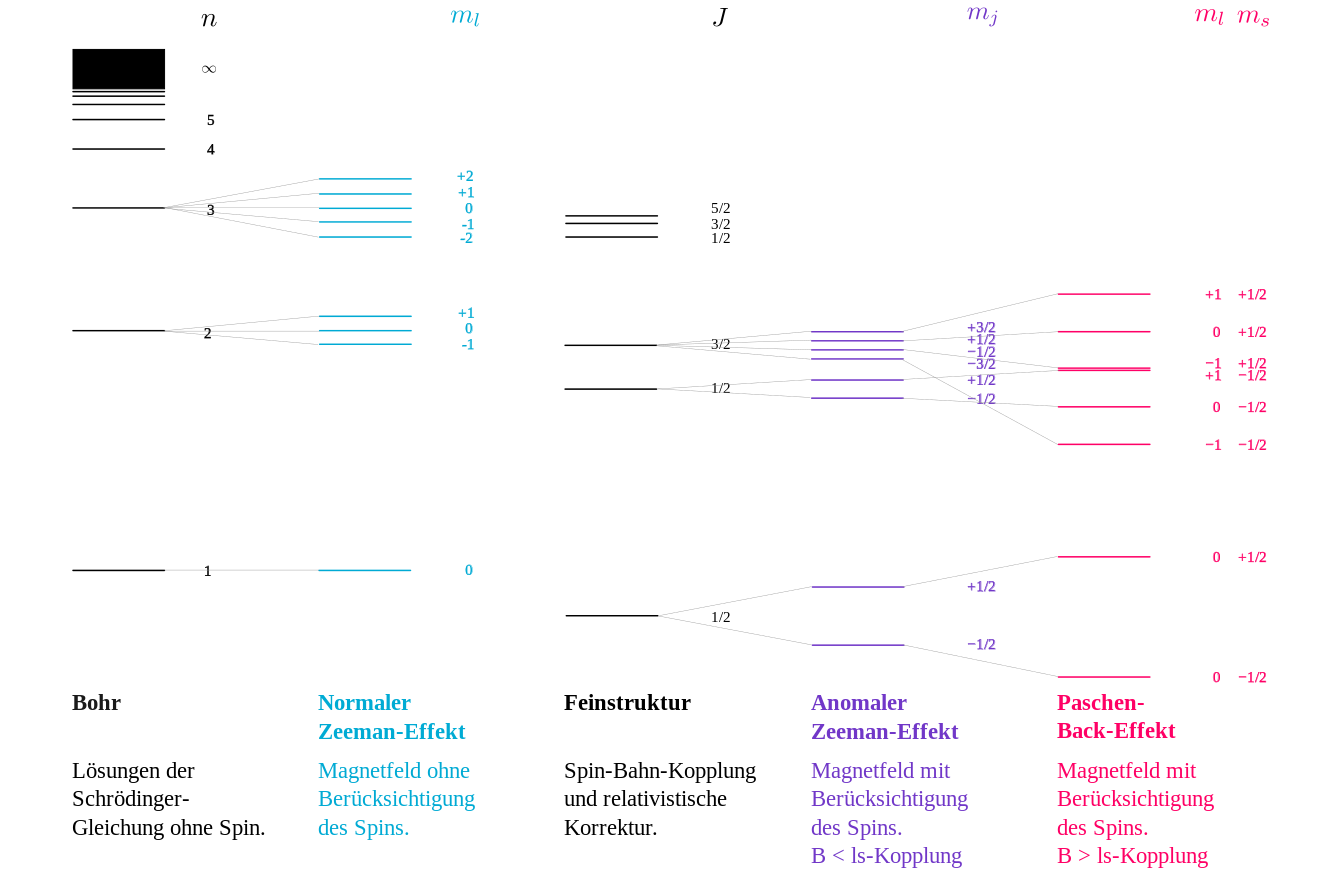
\includegraphics[width=7cm]{Bilddateien/Wasserstoff_Zeeman.svg.png}
            \caption{Aufspaltung der Spektrallinien des Wasserstoffatoms im Magnetfeld.}
        \end{figure}

        \begin{figure}
            \centering
            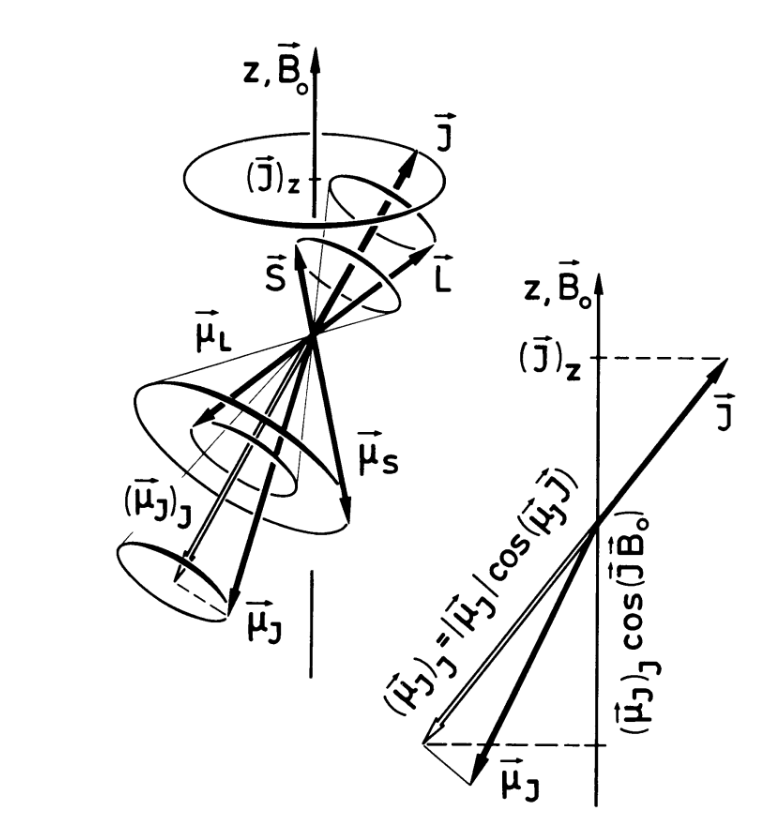
\includegraphics[width=7cm]{Bilddateien/Praezession.png}
            \caption{Präzession der Drehimpulsvektoren von Elektron und Kern.}
        \end{figure}
        \begin{Aufgabe}
            \nr{} Schreibe eine schöne Geschichte zu diesem Thema. [$\to$ Haken-Wolf]

            \nr{} Berechne die zeitliche Mittelung von $\mu_j$. 
        \end{Aufgabe}

\end{document}